\documentclass{article}

\usepackage{amsthm, amsfonts, amsmath, amssymb}
\allowdisplaybreaks[1]

\usepackage{graphicx}
\usepackage{fullpage}
\usepackage{float}
\usepackage{hyperref}

\newtheorem{lemma}{Lemma}
\newtheorem{theorem}{Theorem}
\newtheorem{corollary}{Corollary}
\newtheorem{conjecture}{Conjecture}
\newtheorem{definition}{Definition}

\setlength{\parindent}{0em}

\renewcommand{\O}{\mathcal{O}}
\newcommand{\N}{\mathbb{N}}
\newcommand{\xor}{\oplus}

\begin{document}
	\title{A Generalized Approach to the Rank Deficiency of Certain Sized \textit{Lights Out} Boards}
	\author{William Boyles}
	\date{\today}
	\maketitle
	
	\section{Intro}
	In a previous document, we looked at boards of size $g(k) = 2^{k+1} + 2^{k-1} - 1$ for some natural number $k$.
	We can equivalently write $g(k) = 5\cdot2^{k-1} - 1$.
	We can thus generalize $g$ by allowing the leading coefficient to vary so we get
	\begin{equation*}
		g(b,k) = b\cdot2^{k-1} - 1.
	\end{equation*}
	We restrict $b$ to be odd as we want to maximize $k$.
	In the $b=5$ case, we were able to prove a general form of the Chebyshev polynomials for these board sizes and find the degree of their gcd.
	Thus, we were able to derive the rank deficiency of boards sized $g(5,k) \times g(5,k)$.
	We also conjectured that these boards represented exactly the highest rank deficiencies.
	In the next sections, we will investigate different values of $b$ and make conjectures about the corresponding Chebyshev polynomials and the rank deficiencies.
	
	First, we'll notice that every natural number can be represented in this form.
	\begin{lemma}
		Let $n \in \N$.
		Then $n$ can be represented in the form $b\cdot2^{k-1}$ where $b \in \N$ is odd and $k \in \N$.
	\end{lemma}
	\begin{proof}
		Since 2 is a prime, we can represent any natural number uniquely as $n = b\cdot2^{k-1}$, where $b$ is an odd natural and $k \in \N$.
	\end{proof}
	This proof also gives us a way to find $b$ and $k$ for any $n$: Simply divide by 2 as many times as possible. The number of times you divided is $k-1$, and the odd number you're left with is $b$.
	If we were to represent $n$ in binary, $b$ would be all the digits from the first 1 to the last 1, and $k-1$ would be the number of trailing 0's after the last 1.
	
	\newpage
	\section{When $b = 1$}
	If $b=1$, then $g(1,k) = 2^{k-1} - 1$.
	Below is a table of the Chebyshev polynomials for various values of $k$ and their gcd.
	
	\begin{table}[H]
		\renewcommand{\arraystretch}{1.5}
		\centering
		\begin{tabular}{|l||l|l|l|}
			\hline
			$k$ & $f(g(1,k),x)$ & $f(g(1,k),x+1)$ & $\gcd$  \\
			\hline\hline
			1 & $1$ & $1$ & $1$ \\
			\hline
			2 & $x$ & $x+1$ & $1$ \\
			\hline
			3 & $x^3$ & $x^3+x^2+x+1$ & $1$ \\
			\hline
			4 & $x^7$ & $x^7 + x^6 + \dots + x + 1$ & $1$ \\
			\hline
			5 & $x^{15}$ & $x^{15} + x^{14} + \dots + x + 1$ & $1$ \\
			\hline
			6 & $x^{31}$ & $x^{31} + x^{30} + \dots + x + 1$ & $1$ \\
			\hline
			7 & $x^{63}$ & $x^{63} + x^{62} + \dots + x + 1$ & $1$ \\
			\hline
			8 & $x^{127}$ & $x^{127} + x^{126} + \dots + x + 1$ & $1$ \\
			\hline  
		\end{tabular}
	\end{table}
	Thus, we conjecture
	\begin{conjecture}
		Let $k \in \N$.
		Then the following are true:
		\begin{enumerate}
			\item
			\begin{equation*}
				f(g(1,k),x) = x^{g(1,k)}
			\end{equation*}
			\item
			\begin{equation*}
				f(g(1,k),x+1) = \sum_{n=0}^{g(1,k)}{x^n}
			\end{equation*}
			\item
			\begin{equation*}
				\gcd\left({f(g(1,k),x), f(g(1,k),x+1)}\right) = 1.
			\end{equation*}
		\end{enumerate}
	\end{conjecture}
	This conjecture implies that the nullity of all boards of size $g(1,k) \times g(1,k)$ is $0$.
	This is consistent with empirical evidence. \\
	
	Notice that 1 implies 2 because
	\begin{align*}
		f(g(1,k),x) &= x^{g(1,k)} \\
		f(g(1,k),x+1) &= (x+1)^{g(1,k)} \\
			&= \frac{(x+1)^{2^{k-1}}}{x+1} \\
			&\equiv \frac{x^{2^{k-1}}+1}{x+1} \\
			&\equiv \frac{1-x^{2^{k-1}}}{1-x} \\
			&= 1 + \dots + x^{g(1,k)}.
	\end{align*}
	
	It's not too difficult to see in this case that statements 1 and 2 together imply statement 3.
	Thus, we only need to prove statement 1 true to prove the conjecture.
	
	\newpage
	\section{When $b = 3$}
	If $b=3$, then $g(3,k) = 3\cdot2^{k-1} - 1$.
	Below is a table of the Chebyshev polynomials for various values of $k$ and their gcd.
	
	\begin{table}[H]
		\renewcommand{\arraystretch}{1.5}
		\centering
		\begin{tabular}{|l||l|l|l|}
			\hline
			$k$ & $f(g(3,k),x)$ & $f(g(3,k),x+1)$ & $\gcd$  \\
			\hline\hline
			1 & $x^2 + 1$ & $x^2$ & $1$ \\
			\hline
			2 & $x^5 + x$ & $x^5 + x^4$ & $x^2 + x$ \\
			\hline
			3 & $x^{11} + x^3$ & $x^{11} + x^{10} + x^9 + x^8$ & $x^6 + x^5 + x^4 + x^3$ \\
			\hline
			4 & $x^{23} + x^{7}$ & $x^{23} + \dots + x^{16}$ & $x^{14} + \dots + x^7$ \\
			\hline
			5 & $x^{47} + x^{15}$ & $x^{47} + \dots + x^{32}$ & $x^{30} + \dots + x^{15}$ \\
			\hline
			6 & $x^{95} + x^{31}$ & $x^{95} + \dots + x^{64}$ & $x^{62} + \dots + x^{31}$ \\
			\hline
			7 & $x^{191} + x^{63}$ & $x^{191} + \dots + x^{128}$ & $x^{126} + \dots + x^{63}$ \\
			\hline
			8 & $x^{383} + x^{127}$ & $x^{383} + \dots + x^{256}$ & $x^{254} + \dots + x^{127}$ \\
			\hline  
		\end{tabular}
	\end{table}
	Thus, we conjecture
	\begin{conjecture}
		Let $k \in \N$.
		Then the following are true:
		\begin{enumerate}
			\item
			\begin{equation*}
				f(g(3,k),x) = x^{g(3,k)} + x^{g(1,k)}.
			\end{equation*}
			\item
			\begin{equation*}
				f(g(3,k),x+1) = \sum_{n=2^k}^{g(3,k)}{x^n} = x^{2^k}\sum_{n=0}^{g(1,k)}{x^n}.
			\end{equation*}
			\item
			\begin{equation*}
				\gcd\left({f(g(1,k),x), f(g(1,k),x+1)}\right) = \sum_{n=g(1,k)}^{2g(1,k)}{x^n} = x^{g(1,k)}\sum_{n=0}^{g(1,k)}{x^n}.
			\end{equation*}
		\end{enumerate}
	\end{conjecture}
	This conjecture implies that the nullity of all boards of size $g(3,k) \times g(3,k)$ is $2g(1,k)$.
	This is consistent with empirical evidence. \\
	
	Notice that 1 implies 2 because
	\begin{align*}
		f(g(3,k),x) &= x^{3\cdot2^{k-1}-1} + x^{2^{k-1}-1} \\
		f(g(3,k),x+1) &= (x+1)^{3\cdot2^{k-1}-1} + (x+1)^{2^{k-1}-1} \\
		&= \frac{1}{x+1}\left((x+1)^{3\cdot2^{k-1}} + (x+1)^{2^{k-1}}\right) \\
		&= \frac{1}{x+1}\left(\left((x+1)^{2^{k-1}}\right)^3 + (x+1)^{2^{k-1}}\right) \\
		&\equiv \frac{1}{x+1}\left(\left(x^{2^{k-1}}+1\right)^3 + x^{2^{k-1}} + 1\right) \\
		&= \frac{1}{x+1}\left(\left(x^{2^{k-1}}+1\right)^2\left(x^{2^{k-1}}+1\right) + x^{2^{k-1}} + 1\right) \\
		&\equiv \frac{1}{x+1}\left(\left(x^{2\cdot2^{k-1}}+1\right)\left(x^{2^{k-1}}+1\right) + x^{2^{k-1}} + 1\right) \\
		&= \frac{1}{x+1}\left(x^{3\cdot2^{k-1}} + x^{2^{k-1}} + x^{2\cdot2^{k-1}} + 1 + x^{2^{k-1}} + 1\right) \\
		&\equiv \frac{1}{x+1}\left(x^{3\cdot2^{k-1}} + x^{2\cdot2^{k-1}}\right) \\
		&= \frac{x^{2^{k}}}{x+1}\left(x^{2^{k-1}} + 1\right) \\
		&\equiv x^{2^{k}}\frac{1-x^{2^{k-1}}}{1-x} \\
		&= x^{2^{k}}\left(x^{2^{k-1}-1}+x^{2^{k-1}-2}+\dots+x+1\right) \\
		&= x^{3\cdot2^{k-1}-1} + x^{3\cdot2^{k-1}-2} + \dots + x^{2^k + 1} + x^{2^k} \\
		&= x^{2^k}\sum_{n=0}^{g(1,k)}{x^n}.
	\end{align*}

%	We can use mathematical tools to show that statements 1 and 2 together imply statement 3.

	\newpage
	\section{When $b = 5$}
	We already covered this specific case in another work.
	The main result is that the degree of the GCD of the polynomials is $2^{k+1}$.
	However, for completeness, we'll list out some values in a table and state the conjecture.
	
	\begin{table}[H]
		\renewcommand{\arraystretch}{1.5}
		\centering
		\begin{tabular}{|l||l|l|l|}
			\hline
			$k$ & $f(g(5,k),x)$ & $f(g(5,k),x+1)$ & $\gcd$  \\
			\hline\hline
			1 & $x^4 + x^2 + 1$ & $x^4 + x^2 + 1$ & $x^4 + x^2 + 1$ \\
			\hline
			2 & $x^9 + x^5 + x$ & $\left(x^9 + x^8\right) + \left(x^5 + x^4\right) + \left(x + 1\right)$ & $x^8 + x^4 + 1$ \\
			\hline
			3 & $x^{19} + x^{11} + x^3$ & $\left(x^{19}+\dots+x^{16}\right)+\left(x^{11}+\dots+x^{8}\right)+\left(x^{3}+\dots+1\right)$ & $x^{16} + x^8 + 1$ \\
			\hline
			4 & $x^{39} + x^{23} + x^{7}$ & $\left(x^{39}+\dots+x^{32}\right)+\left(x^{23}+\dots+x^{16}\right)+\left(x^{7}+\dots+1\right)$ & $x^{32} + x^{16} + 1$\\
			\hline
			5 & $x^{79} + x^{47} + x^{15}$ & $\left(x^{79}+\dots+x^{64}\right)+\left(x^{47}+\dots+x^{32}\right)+\left(x^{15}+\dots+1\right)$ & $x^{64} + x^{32} + 1$ \\
			\hline
			6 & $x^{159} + x^{95} + x^{31}$ & $\left(x^{159}+\dots+x^{128}\right)+\left(x^{95}+\dots+x^{64}\right)+\left(x^{31}+\dots+1\right)$ & $x^{128} + x^{64} + 1$\\
			\hline
			7 & $x^{319} + x^{191} + x^{63}$ & $\left(x^{319}+\dots+x^{256}\right)+\left(x^{191}+\dots+x^{128}\right)+\left(x^{63}+\dots+1\right)$ & $x^{256} + x^{128} + 1$ \\
			\hline
			8 & $x^{639} + x^{383} + x^{127}$ & $\left(x^{639}+\dots+x^{512}\right)+\left(x^{383}+\dots+x^{256}\right)+\left(x^{127}+\dots+1\right)$ & $x^{512} + x^{256} + 1$ \\
			\hline
		\end{tabular}
	\end{table}

	Thus, we've conjecture (and subsequently proved)
	\begin{lemma}
		Let $k \in \N$.
		Then the following are true:
		\begin{enumerate}
			\item
			\begin{equation*}
				f(g(5,k),x) = x^{g(5,k)} + x^{g(3,k)} + x^{g(1,k)}.
			\end{equation*}
			\item
			\begin{equation*}
				f(g(5,k),x+1) = \sum_{m\in\{1,3,5\}}{\sum_{n=0}^{g(1,k)}{x^{g(m,k)-n}}}.
			\end{equation*}
			\item
			\begin{equation*}
				\gcd\left(f(g(5,k),x), f(g(5,k),x+1)\right) = \sum_{m\in\{1,3,5\}}{x^{g(m,k)-g(1,k)}}.
			\end{equation*}
		\end{enumerate}
	\end{lemma}
	This lemma implies implies that the nullity of all boards of size $g(5,k) \times g(5,k)$ is $2^{k+1}$.
	This is consistent (as it must be if proven true) with empirical evidence.
	
	\newpage
	\section{When $b = 7$}
	If $b=7$, then $g(7,k) = 7\cdot2^{k-1}-1$.
	Below is a table of the Chebyshev polynomials for various values of $k$ and their gcd.
	
	\begin{table}[H]
		\renewcommand{\arraystretch}{1.5}
		\centering
		\begin{tabular}{|l||l|l|l|}
			\hline
			$k$ & $f(g(7,k),x)$ & $f(g(7,k),x+1)$ & $\gcd$  \\
			\hline\hline
			1 & $x^6 + x^4 + 1$ & $x^6 + x^2 + 1$ & $1$ \\
			\hline
			2 & $x^{13} + x^9 + x$ & $\left(x^{13} + x^{12}\right) + \left(x^{5} + x^{4}\right) + \left(x + 1\right)$ & $1$ \\
			\hline
			3 & $x^{27} + x^{19} + x^3$ & $\left(x^{27} + \dots + x^{24}\right) + \left(x^{11} + \dots + x^8\right) + \left(x^3 \dots + 1\right)$ & $1$ \\
			\hline
			4 & $x^{55} + x^{39} + x^7$ & $\left(x^{55}+\dots+x^{48}\right)+\left(x^{23}+\dots+x^{16}\right)+\left(x^7+\dots+1\right)$ & $1$ \\
			\hline 
			5 & $x^{111} + x^{79} + x^{15}$ & $\left(x^{111}+\dots+x^{96}\right)+\left(x^{57}+\dots+x^{32}\right)+\left(x^{15}+\dots+1\right)$ & $1$ \\
			\hline
			6 & $x^{223} + x^{159} + x^{31}$ & $\left(x^{223}+\dots+x^{192}\right)+\left(x^{115}+\dots+x^{64}\right)+\left(x^{31}+\dots+1\right)$ & $1$ \\
			\hline
			7 & $x^{447} + x^{319} + x^{63}$ & $\left(x^{447}+\dots+x^{384}\right)+\left(x^{231}+\dots+x^{128}\right)+\left(x^{63}+\dots+1\right)$ & $1$ \\
			\hline
			8 & $x^{895} + x^{639} + x^{127}$ & $\left(x^{895}+\dots+x^{768}\right)+\left(x^{463}+\dots+x^{256}\right)+\left(x^{127}+\dots+1\right)$ & $1$ \\
			\hline
		\end{tabular}
	\end{table}

	Thus, we conjecture
	\begin{conjecture}
		Let $k \in \N$.
		Then the following are true:
		\begin{enumerate}
			\item
			\begin{equation*}
				f(g(7,k),x) = x^{g(7,k)} + x^{g(5,k)} + x^{g(1,k)}.
			\end{equation*}
			\item
			\begin{equation*}
				f(g(7,k),x+1) = \sum_{m\in\{1,3,7\}}{\sum_{n=0}^{g(1,k)}{x^{g(m,k)-n}}}
			\end{equation*}
			\item
			\begin{equation*}
				\gcd\left(f(g(7,k),x),f(g(7,k),x+1)\right) = 1.
			\end{equation*}
		\end{enumerate}
	\end{conjecture}
	This conjecture implies that the nullity of all boards of size $g(7,k) \times g(7,k)$ is 0.
	This is consistent with empirical evidence. \\
	
	Notice that statement 1 implies statement 2 because
	\begin{align*}
		f(g(7,k),x) &= x^{g(7,k)} + x^{g(5,k)} + x^{g(1,k)} \\
		f(g(7,k),x+1) &= (x+1)^{g(7,k)} + (x+1)^{g(5,k)} + (x+1)^{g(1,k)} \\
		%&= (x+1)^{7\cdot2^{k-1}-1} + (x+1)^{5\cdot2^{k-1}-1} + (x+1)^{2^{k-1}-1} \\
		&= \frac{1}{x+1} \left((x+1)^{7\cdot2^{k-1}} + (x+1)^{5\cdot2^{k-1}} + (x+1)^{2^{k-1}}\right) \\
		&= \frac{(x+1)^{2^{k-1}}}{x+1}\left((x+1)^{4\cdot2^{k-1}}(x+1)^{2\cdot2^{k-1}}+(x+1)^{4\cdot2^{k-1}}+1\right) \\
		&\equiv \frac{x^{2^{k-1}}+1}{x+1}\left(\left(x^{4\cdot2^{k-1}}+1\right)\left(x^{2\cdot2^{k-1}}+1\right)+\left(x^{4\cdot2^{k-1}}+1\right)+1\right) \\
		&\equiv \frac{1-x^{2^{k-1}}}{1-x}\left(x^{6\cdot2^{k-1}}+x^{4\cdot2^{k-1}}+x^{2\cdot2^{k-1}}+1+x^{4\cdot2^{k-1}}+1+1\right) \\
		&\equiv \frac{1-x^{2^{k-1}}}{1-x}\left(x^{6\cdot2^{k-1}}+x^{2\cdot2^{k-1}}+1\right) \\
		&= \left(1+\dots+x^{2^{k-1}-1}\right)\left(x^{6\cdot2^{k-1}}+x^{2\cdot2^{k-1}}+1\right) \\
		&= \left(x^{6\cdot2^{k-1}}+\dots+x^{7\cdot2^{k-1}-1}\right) + \left(x^{2\cdot2^{k-1}}+\dots+x^{3\cdot2^{k-1}-1}\right) + \left(1+\dots+x^{2^{k-1}-1}\right) \\
		&= \sum_{m\in\{1,3,7\}}{\sum_{n=0}^{g(1,k)}{x^{g(m,k)-n}}}.
	\end{align*}
	
	\newpage
	\section{When $b = 9$}
	If $b=9$, then $g(9,k) = 9\cdot2^{k-1} - 1$.
	Below is a table of Chebyshev polynomials for various values of $k$ and their GCD.
	
	\begin{table}[H]
		\renewcommand{\arraystretch}{1.5}
		\begin{tabular}{|l||l|l|l|}
			\hline
			$k$ & $f(g(9,k),x)$ & $f(g(9,k),x+1)$ & $\gcd$ \\
			\hline \hline
			1 & $x^8 + x^6 + x^4 + 1$ & $x^8 + x^6 + x^2$ & $1$ \\
			\hline
			2 & $x^{17} + x^{13} + x^{9} + x$ & $\left(x^{17} + x^{16}\right) + \left(x^{13} + x^{12}\right) + \left(x^{5} + x^{4}\right)$ & $x^2 + x$ \\
			\hline
			3 & $x^{35} + x^{27} + x^{19} + x^{3}$ & $\left(x^{35}+\dots+x^{32}\right)+\left(x^{27}+\dots+x^{24}\right)+\left(x^{11}+\dots+x^8\right)$& $x^6 + x^5 + x^4 + x^3$ \\
			\hline
			4 & $x^{71} + x^{55} + x^{39} + x^{7}$ & $\left(x^{71}+\dots+x^{64}\right)+\left(x^{55}+\dots+x^{48}\right)+\left(x^{23}+\dots+x^{16}\right)$ & $x^{14} + \dots + x^7$ \\
			\hline
			5 & $x^{143} + x^{111} + x^{79} + x^{15}$ & $\left(x^{143}+\dots+x^{128}\right)+\left(x^{111}+\dots+x^{96}\right)+\left(x^{57}+\dots+x^{32}\right)$ & $x^{30} + \dots + x^{15}$ \\
			\hline
			6 & $x^{287} + x^{223} + x^{159} + x^{31}$ & $\left(x^{287}+\dots+x^{256}\right)+\left(x^{223}+\dots+x^{192}\right)+\left(x^{115}+\dots+x^{64}\right)$ & $x^{62} + \dots + x^{31}$ \\
			\hline
			7 & $x^{757} + x^{447} + x^{319} + x^{63}$ & $\left(x^{757}+\dots+x^{512}\right)+\left(x^{447}+\dots+x^{384}\right)+\left(x^{231}+\dots+x^{128}\right)$ & $x^{126} + \dots + x^{63}$ \\
			\hline
			8 & $x^{1515} + x^{895} + x^{639} + x^{127}$ & $\left(x^{1515}+\dots+x^{1024}\right)+\left(x^{895}+\dots+x^{768}\right)+\left(x^{463}+\dots+x^{256}\right)$ & $x^{254} + \dots + x^{127}$ \\
			\hline
		\end{tabular}
	\end{table}

	Thus, we conjecture
	\begin{conjecture}
		Let $k \in \N$.
		Then the following are true:
		\begin{enumerate}
			\item
			\begin{equation*}
				f(g(9,k),x) = x^{g(9,k)} + x^{g(7,k)} + x^{g(5,k)} + x^{g(1,k)}.
			\end{equation*}
			\item
			\begin{equation*}
				f(g(9,k),x+1) = \sum_{m\in\{3,7,9\}}{\sum_{n=0}^{g(1,k)}{x^{g(m,k)-n}}}.
			\end{equation*}
			\item
			\begin{equation*}
				\gcd\left(f(g(9,k),x),f(g(9,k),x+1)\right) = x^{g(1,k)}\sum_{n=0}^{g(1,k)}{x^n}.
			\end{equation*}
		\end{enumerate}
	\end{conjecture}
	This conjecture implies that the nullity of all boards of size $g(9,k) \times g(9,k)$ is $2g(1,k)$.
	This is consistent with empirical evidence. \\
	
	Notice that statement 1 implies statement 2 because
	\begin{align*}
		f(g(9.k),x) &= x^{g(9,k)} + x^{g(7,k)} + x^{g(5,k)} + x^{g(1,k)} \\
		f(g(9,k),x+1) &= (x+1)^{g(9,k)} + (x+1)^{g(7,k)} + (x+1)^{g(5,k)} + (x+1)^{g(1,k)} \\
		&= \frac{1}{x+1}\left((x+1)^{9\cdot2^{k-1}} + (x+1)^{7\cdot2^{k-1}} + (x+1)^{5\cdot2^{k-1}} + (x+1)^{2^{k-1}}\right) \\
		&= \frac{(x+1)^{2^{k-1}}}{x+1}\left((x+1)^{8\cdot2^{k-1}} + (x+1)^{4\cdot2^{k-1}}(x+1)^{2\cdot2^{k-1}} + (x+1)^{4\cdot2^{k-1}} + 1\right) \\
		&\equiv \frac{x^{2^{k-1}}+1}{x+1}\left(\left(x^{8\cdot2^{k-1}}+1\right) + \left(x^{4\cdot2^{k-1}}+1\right)\left(x^{2\cdot2^{k-1}}+1\right) + \left(x^{4\cdot2^{k-1}}+1\right) + 1\right) \\
		&\equiv \frac{1-x^{2^{k-1}}}{1-x}\left(x^{8\cdot2^{k-1}} + 1 + x^{6\cdot2^{k-1}} + x^{4\cdot2^{k-1}} + x^{2\cdot2^{k-1}} + 1 + x^{4\cdot2^{k-1}} + 1 + 1\right) \\
		&\equiv \frac{1-x^{2^{k-1}}}{1-x}\left(x^{8\cdot2^{k-1}}+x^{6\cdot2^{k-1}}+x^{2\cdot2^{k-1}}\right) \\
		&= \left(1+\dots+x^{2^{k-1}-1}\right)\left(x^{8\cdot2^{k-1}}+x^{6\cdot2^{k-1}}+x^{2\cdot2^{k-1}}\right) \\
		&= \left(x^{8\cdot2^{k-1}}+\dots+x^{9\cdot2^{k-1}-1}\right) + \left(x^{6\cdot2^{k-1}}+\dots+x^{7\cdot2^{k-1}-1}\right) + \left(x^{2\cdot2^{k-1}}+\dots+x^{3\cdot2^{k-1}-1}\right) \\
		&= \sum_{m\in\{3,7,9\}}{\sum_{n=0}^{g(1,k)}{x^{g(m,k)-n}}}.
	\end{align*}
	Also, notice that we have the same conjectured GCD result here as for $b=3$.
	In fact, we can somewhat ``see'' the parts from $b=3$ in our table.
	The last grouping of terms in the $f(g(9,k),x+1)$ column are exactly the same terms as in the entire $f(g(3,k),x+1)$ column.

	\newpage
	\section{Meta-Conjectures}
	Now that we've seen many examples of how these polynomials and their GCDs because for various values of $b$ and $k$, we'll make some conjectures concerning the more general behavior of such polynomials.
	
	\begin{conjecture}
		Let
		\begin{equation*}
			f(g(b,k),x) = x^{n_1} + x^{n_2} + \dots + x^{n_m}.
		\end{equation*}
		Then
		\begin{equation*}
			f(g(b,k+1),x) = x^{2n_1 + 1} + x^{2n_2 + 1} + \dots + x^{2n_m + 1}.
		\end{equation*}
	\end{conjecture}
	This implies that if we know the exponents of $f(g(b,1),x)$, we can iteratively calculate them for any $f(g(b,k),x)$.
	
	We can also establish a corollary that seems to have an interesting connection to another part of mathematics.
	\begin{corollary}
		For a fixed value of $b$, the number of non-zero terms in $f(g(b,k),x)$ is the same for all $k$.
	\end{corollary}
	Below is a table of various values of $b$ and the number of non-zero terms in $f(g(b,k),x)$.
	
	\begin{table}[H]
		\centering
		\begin{tabular}{|l||l|}
			\hline
			$b$ & Number of Non-Zero Terms in $f(g(b,k),x)$ \\
			\hline\hline
			1 & 1 \\
			\hline
			3 & 2 \\
			\hline
			5 & 3 \\
			\hline
			7 & 3 \\
			\hline
			9 & 4 \\
			\hline
			11 & 5 \\
			\hline
			13 & 5 \\
			\hline
			15 & 4 \\
			\hline
			17 & 5 \\
			\hline
			19 & 7 \\
			\hline
			21 & 8 \\
			\hline
			23 & 7 \\
			\hline
			25 & 7 \\
			\hline
			27 & 8 \\
			\hline
			29 & 7 \\
			\hline
		\end{tabular}
	\end{table}
	
	Putting this sequence into the OEIS, we see that it matches with \href{https://oeis.org/A007306}{A007306}, which are the denominators of Farey tree fractions, which is pictured below.
	We can see that the sequence is simply the denominators of the tree read level by level, left to right.
	
	\begin{figure}[H]
		\centering
		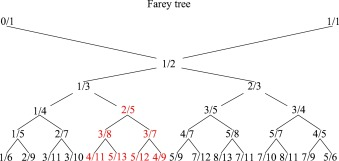
\includegraphics[width=0.8\textwidth]{farey_tree.jpg}
		\caption{Farey Tree in range [0,1]. Also known as Stern-Brocot Tree.}
	\end{figure}

	\begin{conjecture}
		Choose any $b \in \N$ odd and $k \in \N$.
		Let
		\begin{equation*}
			f(g(b,k),x+1) = x^{n_1} + x^{n_2} + \dots + x^{n_m}.
		\end{equation*}
		Then
		\begin{equation*}
			f(g(b,k+1),x+1) = x^{2n_1 + 1} + x^{2n_1} + x^{2n_2 + 1} + x^{2n_2} + \dots + x^{2n_m + 1} + x^{2n_m}.
		\end{equation*}
	\end{conjecture}
	This implies that if we know the exponents of $f(g(b,1),x+1)$, we can iteratively calculate them for any $f(g(b,k),x+1)$.
	
	Like previously, we can establish a corollary about the number of non-zero terms.
	\begin{corollary}
		Choose any $b \in \N$ odd and $k \in \N$.
		Then the number of non-zero terms in $f(g(b,k),x+1)$ is $2^{k-1}$ times as many non-zero terms as in $f(g(b,1),x+1)$.
	\end{corollary}
	Notice that means we can write the number of non-zero terms in $f(g(b,k),x+1)$ as $g(b',k)$, where $b'$ is the number of non-zero terms in $f(g(b,1),x+1)$.
	Below is a table of various values of $b$ and the number of non-zero terms in $f(g(b,1),x+1)$.
	
	\begin{table}[H]
		\centering
		\begin{tabular}{|l||l|}
			\hline
			$b$ & Number of Non-Zero Terms in $f(g(b,1),x+1)$ \\
			\hline\hline
			1 & 1 \\
			\hline
			3 & 1 \\
			\hline
			5 & 3 \\
			\hline
			7 & 3 \\
			\hline
			9 & 3 \\
			\hline
			11 & 3 \\
			\hline
			13 & 5 \\
			\hline
			15 & 5 \\
			\hline
			17 & 7 \\
			\hline
			19 & 7 \\
			\hline
			21 & 5 \\
			\hline
			23 & 5 \\
			\hline
			25 & 5 \\
			\hline
			27 & 5 \\
			\hline
			29 & 11 \\
			\hline
		\end{tabular}
	\end{table}
	Although just taking the list of these terms doesn't yield anything in the OEIS, we can find something if we look for sequences whose odd terms are in our table.
	Particularly, it seems that \href{https://oeis.org/A283324}{A283324} is what we want.
	However, we find that this sequence represents the cellular automaton that we already knew this sequence came from.

	\begin{conjecture}
		Let $b \in \N$ odd and $k \in \N$. 
		Then the lowest degree term of $\gcd\left(f(g(b,k),x),f(g(b,k),x+1)\right)$ has a degree that is one less than a power of 2.
	\end{conjecture}

	\begin{conjecture}
		Let $b \in \N$ odd and $k \in \N$.
		If $\gcd\left(f(g(b,k),x),f(g(b,k),x+1)\right)$ has a varying amount of terms as $k$ varies with $b$ fixed, then the GCD is a geometric series with some power of 2 number of terms.
	\end{conjecture}
\end{document}